%----------------------------------------------------------------------------
\chapter{Létező eszközök vizsgálata}
%----------------------------------------------------------------------------


Ebben a fejezetben először elterjedt diagram és dokumentum szerkesztő alkalmazásokat mutatok be, emellett webes programfejlesztő alkalmazásokat is. A második felében néhány megvizsgált vizuális programozási nyelv következik.

\section{Diagram és kódszerkesztő webalkalmazások}

%----------------------------------------------------------------------------
\subsection{Lucidcharts}
%----------------------------------------------------------------------------

Lucidchart egy HTML5 és Javascript alapú diagramszerkesztő eszköz.  2008-ban lett béta verzióként elindítva\cite{lucidref}, azóta a teljességre törekedve elég sok modellezési nyelvből lehet már választani: UML diagram típusok nagy része, hálózati diagramok, Venn diagram, kapcsolási rajzok, lakás tervrajz, mind map, okostelefon mockupok és akár folyamatábrát is lehet szerkeszteni.


\begin{figure}[!ht]
\centering
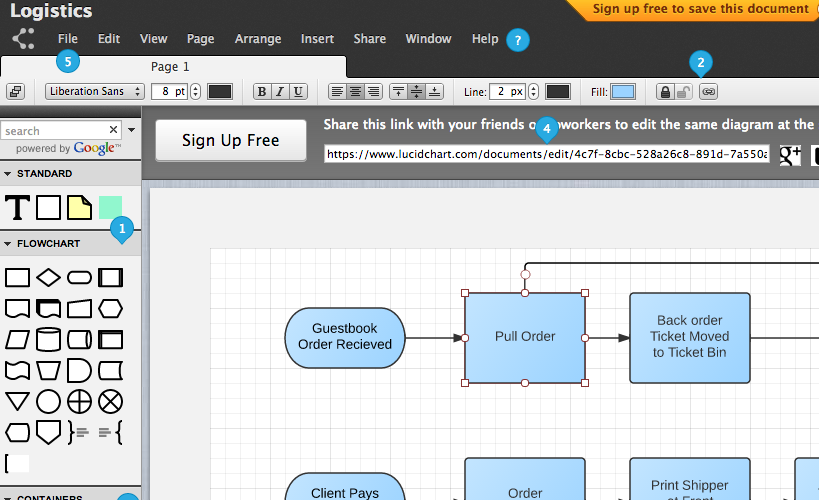
\includegraphics[width=10cm,keepaspectratio]{figures/lucid.png}
\caption{A Lucidchart szerkesztő felülete}
\label{fig:lucideditor}
\end{figure}

A Lucidchart szerkeszőben lehetséges egyszerre módosítani egy diagramot. Kollaborációs szempontból vizsgálva az alkalmazást, a legegyszerűbb eset amit ki lehet próbálni az, hogy két különböző irányba húzza ugyanazt a dobozt két ember és egyszerre engedik el. Nem meglepő, hogy az az eredmény, hogy csak az egyik mozgatás eredménye érvényesül és a másik böngészőben ugyanarra a pozícióra ugrik a doboz. Erre a szituációra a saját alkalmazásomban is ugyanez a viselkedés tapasztalható.

Érdekes megfigyelni, hogy ugyanannak a szövegdoboznak a szerkesztése is kollaboratív: ketten tudnak egyszerre beírni a dobozba és mindkettőnek az eredménye megőrződik. Persze, a doboz kitörlése miatt elveszik az amit éppen beírt a másik felhasználó és aki éppen írt, az nem tudja visszavonni a törlést, mert nem ő törölte. A törlő felhasználó által visszavonva a műveletet nem találjuk meg azt a szöveget amit törlés előtt beleírtak.

Kollaborációs szempontból elég robusztus az alkalmazás, holott nem fed le minden esetet és egy kicsit lassú az események propagálása, sokszor 1-2 másodpercbe is telik, de ez a késés nem befolyásolja az együttműködést jelentősen.

A szerkesztő felület elég barátságos, a nyilakat majdnem akárhova be lehet húzni és tovább lehet állítani a görbék kontroll pontjait, hogy úgy alakítsuk a nyilat ahogy akarjuk. Egy szimpatikus funkció az a Google kép keresés aminek segítségével könnyen berántható a diagramba egy találat.

Diagramszerkesztőként kiváló eszköz, nyomtatható minőségű diagramokat lehet benne létrehozni. Mivel közel tökéletes az alkalmazás erre, nem is ebbe az irányba gondolkoztam, hanem megcéloztam olyan képességet, amire nem képes a Lucidcharts, példáúl a külső rendszerekkel való együttműködés, vagy a diagram felhasználása valamilyen automatizált feldolgozásra. 










 
\subsection{Google Docs}

A Google Docs szerkesztőjében szöveges dokumentumokat, Microsoft Excel típusú táblázatokat, prezentációkat és ábrákat lehet szerkeszteni.

\subsubsection{Kollaboráció a Google Docs-ban}

A Google Docs régebbi verzióiban az egyszerre szerkesztett szövegek a dokumentum verzió számok alapján oldották fel a konfliktusokat\cite{googcoll1}. Laci és Réka szerkesztenek egy dokumentumot szeletet példáúl ``árvíztűrőtükörfúrógép''. Laci a tükör szó betűit dőltté alakítja, ezt a módosítást megkapja a szerver és elküldi Rékának, aki közben kicserélte a tükör szót almára. Ekkor Réka kliensoldalán történik a konfliktus feloldása és az a baj, hogy ``árvíztűrő\emph{alma}fúrógép'' és ``árvíztűrő\emph{tükör}\emph{alma}fúrógép'' mindkettő értelmes feloldás, ha azt gondoljuk, hogy Laci dőlt betűket akart és Réka át akart nevezni.

Ezt továbbfejlesztették verzió alapú feloldás helyett atomi szerkesztési események időrendbeállításával. Az algoritmus neve ``Operational Transformation''\cite{googcoll2} és szöveg bevitel, törlés és stílus módosítás atomi műveleteket fésül össze. A transzformáció része abban áll, hogy egy másik felhasználó módosítását hozzá kell egyeztetni a friss módosításainkhoz. Példáúl adott egy 12 betűs szöveg \lstinline{almabirsalma}, ha Réka törölni akar a végéről két betűt (ma) és közben Laci hozzáír az elejére négy betűt (cica) , akkor Réka \lstinline|{DeleteText 'ma' @11-12}| műveletét Laci \lstinline|{DeleteText 'ma' @15-16}| -ra transzformálja, egyébként \lstinline{cicaalmabialma} lenne az eredmény. Így az eredmény \lstinline{cicaalmabirsal} és mindkét fél szándéka érvényesült.

A stílus módosítás és szövegbevitel összefésülése esetében is történik transzformáció, példáúl, Laci vastagít a 10. és 20. karakterek között: \lstinline|{ApplyStyle bold @10-20}| és Réka közben beleír a közepébe három karaktert: \lstinline|{InsertText 'ABC' @15}|, az eredmény a kettő összefésülése lesz:  \lstinline|{ApplyStyle Bold @10-23}|, vagyis az eredeti szövegrészre vonatkozó stílusváltozás az újra is vonatkozik.

Szöveges dokumentum egyidejű szereksztése estében megjelenik egy beszélgető panel és az alkalmazás színes dobozokkal jelzi, hogy más felhasználó is megnyitotta a dokumentumot. Ezt a funkciót a saját alkalmazásomban is implementáltam a Socket.IO socket szobák segítségével. Megfigyelhető, hogy a többi felhasználó szöveg beviteli kurzora is látszik a felhasználóhoz hozzárendelt színnel kiszínezve. Hozzáadott tartalom esetében, vagy táblázat szerkesztésénél jelezve van, hogy melyik felhasználó éppen mit csinál.

\subsubsection{Diagramszerkesztő}

A diagramszerkesztő alkalmazás viszont sokkal egyszerűbb a Lucidchartsnál. Ez utóbbinál ahhoz, hogy egy nyilat húzzunk egy dobozból elég volt a doboz keretéből egérrel húzni egy másik dobozra és illeszkedett automatikusan a nyíl. A Google Drawing alkalmazásban külön ki kell választani a nyíl eszközt és pontosan a horgonypontjaira kell illeszteni a doboznak ahhoz, hogy a nyíl a dobozhoz legyen kötve és vele együtt mozogjon, ha elhúzzák. A diagramszerkesztő is kollaboratív.

Egy érdekes funkció a vezérvonalak amik segítenek az elemek egymáshoz, vagy az oldal fontos vonalaihoz --példáúl függőleges felezőhöz -- való igazításhoz.

\subsubsection{Verziókezelés}

A dokumentumok előző verziói böngészhetők és visszaállíthatók a \lstinline{Show revision history} paranccsal. A verzió történetben a granularitáson állíthatunk, példáúl csak napi szintű verziózást akarunk látni, vagy annál sűrűbbet.

%----------------------------------------------------------------------------
\subsection{Gliffy}
%----------------------------------------------------------------------------

\begin{figure}[!ht]
\centering
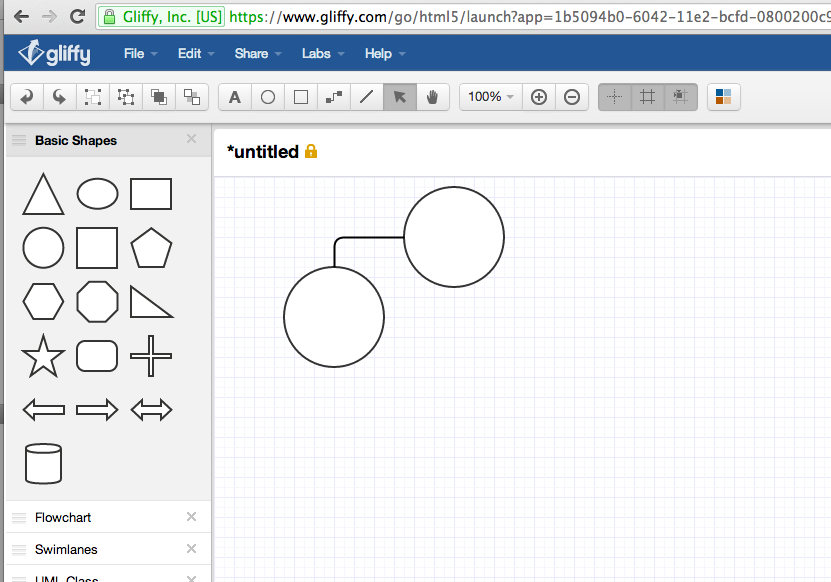
\includegraphics[width=10cm,keepaspectratio]{figures/gliffy.png}
\caption{A Gliffy szerkesztő felülete kiválasztott éllel}
\label{fig:gliffyeditor}
\end{figure}

A Gliffy alkalmazás Lucidcharthoz hasonló diagramszerkesztő, Google Chrome plugin-ként offline üzemmódban is működik, tehát nem csak webes diagramszerkesztő. Habár kevésbé barátságos a nyílhúzó funkciója, egy jó ötlet amit találtam benne az, hogy a kiválasztott elem beállításai elérhetőek az elem mellett közvetlenül egy ablakocskában és nem kell fent keresni az eszköztárban objektumspecifikus beállítást, ahogyan a ~\ref{fig:gliffyeditor} ábrán is látszik. 


\subsection{JSFiddle}

Ezúttal egy programfejlesztő webes alkalmazást mutatok be, a JSFiddle három forrásfájl szerkesztését engedi: HTML, CSS és Javascript forrásfájlok és a futtatás gomb hatására lefut a webalkalmazás amit a 3 forrás alkot. Nagyon jó eszköz prototipizálásra. Gyakran arra használják, hogy hordozható környezetben reprodukáljanak egy hibát és ezt a dokumentumot -- fiddle-nek hívják őket -- elküldve valakinek, az sokkal hamarabban tud segíteni a bajba került kollegának, hiszen megnyitva azonnal látja jelenséget. 

\begin{figure}[!ht]
\centering
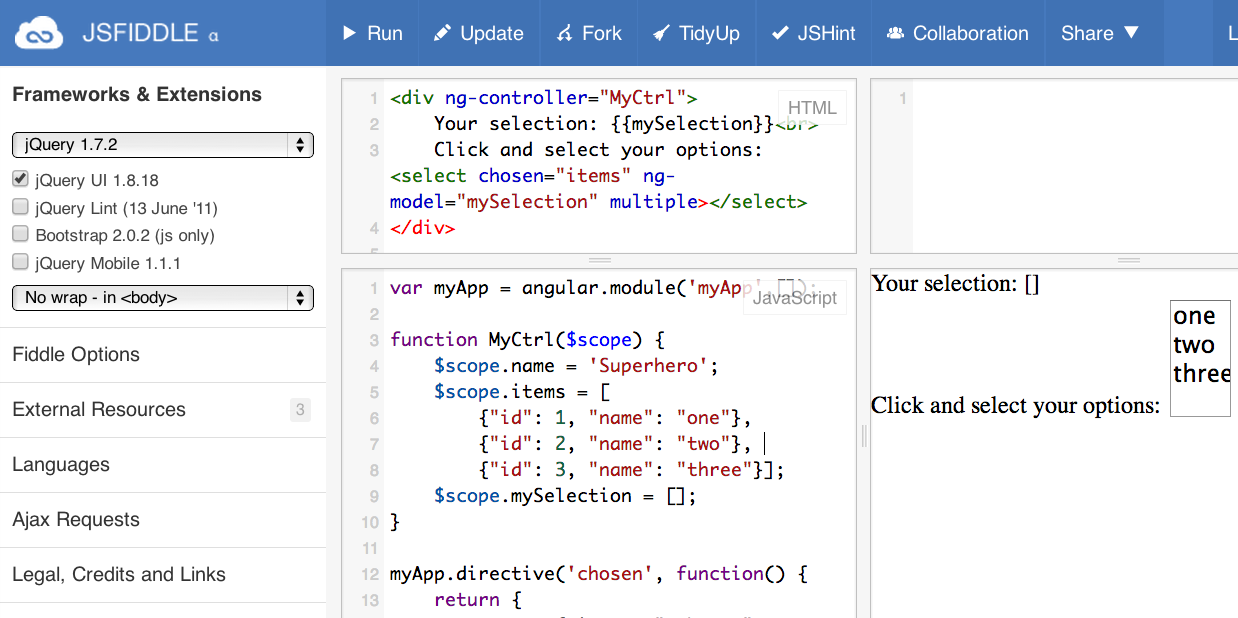
\includegraphics[width=16cm,keepaspectratio]{figures/fiddle.png}
\caption{A JSFiddle szerkesztő}
\label{fig:fiddleeditor}
\end{figure}

JSFiddle alkalmazásokat lehet ``fork''-olni, ami lemásolja őket és új URL-en lehet elérni a friss példányt. Ezt a funkciót én is implementáltam alkalmazásomban.

A JSFiddle érdekes egyrészt azért, mert az alkalmazásomban kódot kell majd szerkeszteni, de azért is, mert ez kollaboratívan is történhet. Az első érdekesség az, hogy mutatja a többi felhasználó egérkurzorának a pozícióját. Sajnos eléggé akadozva történik és előfordulhat, hogy ez inkább zavaró. Kipróbálva azonos szövegrész egyidejű szerkesztését az Operational Transformation példa szerinti művelet -- a mondat eleji írás és mondat végi egyidejű törlése -- észrevettem, hogy hamar elértem, hogy eltérő legyen a két dokumentum, tehát ez alapján lehet arra következtetni, hogy nem Operational Transformation algoritmust használnak az egyidejű szerkesztésre.


%\subsection{CodeWars}

%\begin{figure}[!ht]
%\centering
%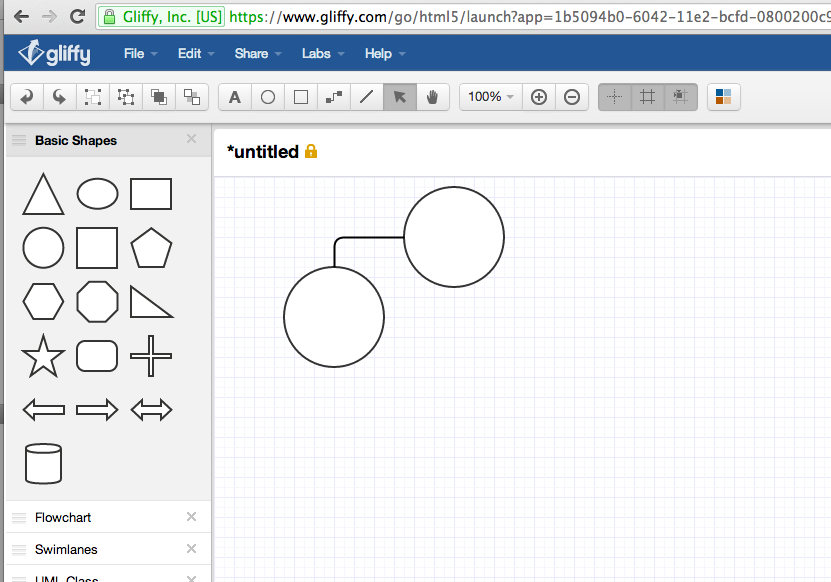
\includegraphics[width=10cm,keepaspectratio]{figures/gliffy.png}
%\caption{A Gliffy szerkesztő felülete kiválasztott éllel}
%\label{fig:warseditor}
%\end{figure}


\section{Vizuális programozási nyelvek}

\subsection{Blockly}

\begin{figure}[!ht]
\centering
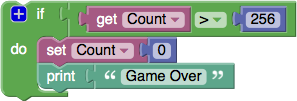
\includegraphics[width=8cm,keepaspectratio]{figures/blockly.png}
\caption{A Blockly vizuális nyelv}
\label{fig:blockly}
\end{figure}

A Blockly nyelvben vizuálisan tudunk összerakni programokat ``puzzle''-szerű elemekből. A dokumentáció szerint ez kedvező kezdő programozóknak, mert ők két próblémával küzdenek: a gondolataikat nehezen fordítják le logikus kijelentésekre és a szintaxissal való küzdés. A Blockly-ben nem lehet a szintaxist elrontani, hiszen csak olyan parancsokat rakhatunk össze amik engedélyezettek a szintaxis szempontjából. Ez egy fontos gondolat vizuális nyelvek felhasználói felületének a kialakításánál -- nem is kell lehetségessé tenni a hibás bemenetet. Sok tanuló fejlesztő egy üres szöveges forrást látva nem tudja hol kezdje el, és a Blockly esetében választhat létező elemekből, ami megkönnyíti helyzetüket\cite{blocklyref}.

Az egyik példa alkalmazás Blockly alapon pont egy Python és Javascript kód generátor, ami lefordítja a diagramot kóddá, ez sejteti az egyik okot amiért nem ilyen jellegű modellezési alkalmazást fejlesztettem: mivel a grafikus változat egy-az-egyben megfelel a generált kódnak, akkor főleg Python esetében, nem indokolt egy tapasztalt fejlesztőnek a grafikus felület használata. Más szóval a grafikus felületet nem arra használjuk Blockly-ban, hogy olyat fejezzünk ki, amit nem lehet, vagy nehéz kódban kifejezni. 

Ellenpélda a vizuális nyelv, amit implementáltam, az állapotgép: ebben az esetben nyilvánvaló ez a gondolat, hiszen egy 25 állapotot tartalmazó állapotgép könnyeben érthető vizuálisan és könnyebben is szerkeszthető kollaboratívan.

%\subsection{NoFlo}

%\begin{figure}[!ht]
%\centering
%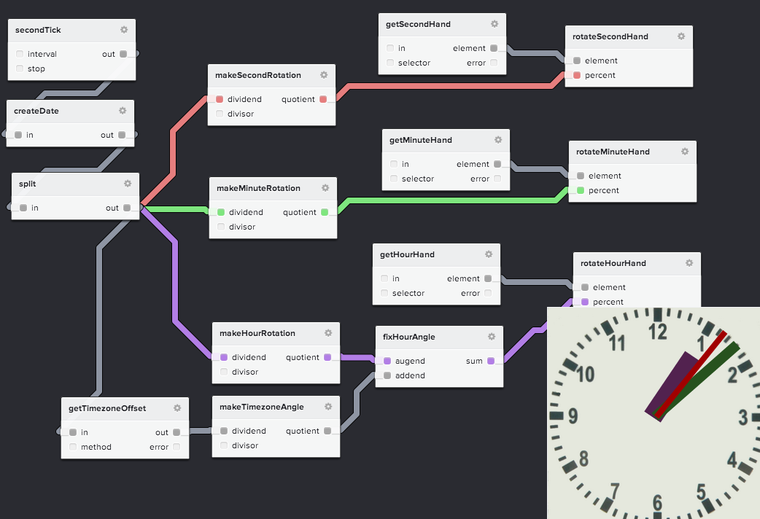
\includegraphics[width=12cm,keepaspectratio]{figures/clock.png}
%\caption{A NoFlo vizuális nyelvben egy órának az implementációja}
%\label{fig:noflo}
%\end{figure}

\section{Összefoglalás}

A prototipizálás során arra jutottam, hogy a rendszernek a két aspektusa --  kollaboratív szerkesztés és vizuális nyelv fejlesztése -- közül nagyobb hangsúlyt szeretnék fektetni az elsőre, emiatt egy egyszerű nyelvet fogok megvalósítani: az állapotgép vizuális nyelvét, viszont a webalkalmazást úgy építem fel, hogy a vizuális nyelv jellege is felhasználó által legyen meghatározható. Ha akarjuk, akkor az abszrakcióban egy szinttel feljebb céloztam: vizuális nyelveket szerkesztő alkalmazás. 

A végső kimenet egy példányosítható osztály, ami egy programot valósít meg, ez a program vizuálisan szerkeszthető, viszont a programozási nyelv változtatható a transzformációs szabályok módosítása által.

